\section{Performance Evaluation}
To evaluate the performance of \sink, we are concerned with (1) the overhead incurred by the semantic translation methods discussed in Section 4, (2) the message latency when crossing between different networks (e.g., the RTT of IP-to-NDN messages), and (3) the latency of messages traversing NDN bridges. Since bridge key generation and directory updates happen infrequently and asynchronously, we did not measure the time to perform these tasks; we leave such evaluation to future work. To assess each of these measurements, we deployed a single bridge directory server that managed four (geographically) remote clients. Each of these hosts were running Ubuntu 12.10 and ran CCNx 0.81 and Python 3.1. Cryptographic libraries such as OpenSSL were not used for MAC tag generation and verification. 

Measurements (1) and (2) were tested via scripts that issue a series of IP-to-NDN and NDN-to-IP requests and record the time to retrieve a response. The overhead of translating IP to NDN messages was approximately 0.00078s for interest names composed of one (1) to five (5) components. Similarly, the overhead of translating NDN to IP messages was slightly higher with an average time of 0.005s. Clearly, this overhead is negligible for sequential requests generated by small loads. Due to a lack of resources, large-scale tests were not conducted to see how this overhead increased with request load. Measurement (3) was tested by two remote clients connected to the central bridge directory. A script running on one client issued a series of NDN interests (via {\tt ccnpeek}) to be forwarded to the other client and satisfied by its set of connected hosts, and the RTT to retrieve content for each invocation of {\tt ccnpeek} was recorded. 

The RTT results for measurements (2) and (3) when retrieving content of roughly 1MB and 10MB in size is shown in Figures \ref{fig:perf1} and \ref{fig:perf2}. Our results indicate that IP-to-NDN and bridge message latencies were fairly consistent, whereas NDN-to-IP content retrieval incurred sporadic spikes in RTT. We attribute these anomalies to Python's thread synchronization primitives. 

\begin{figure}
\begin{center}
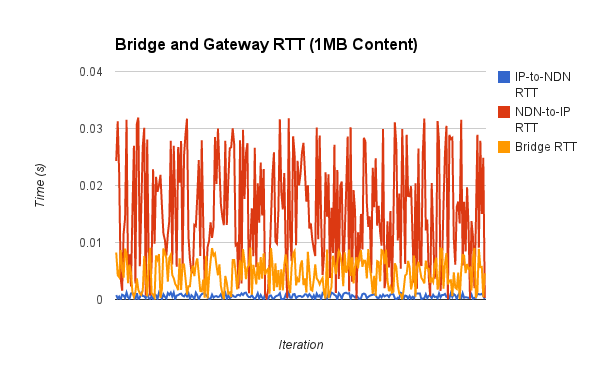
\includegraphics[scale=0.4]{./images/small.png}
\label{fig:perf1}
\caption{Average RTT times for IP-to-NDN, NDN-to-IP, and bridge messages when requesting content of approximately 1MB in size.}
\end{center}
\end{figure}

\begin{figure}
\begin{center}
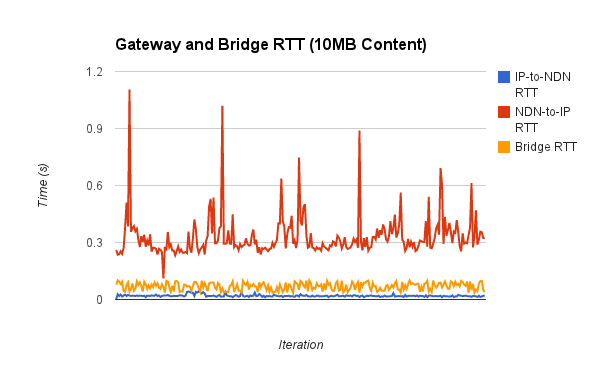
\includegraphics[scale=0.4]{./images/large.png}
\label{fig:perf2}
\caption{Average RTT times for IP-to-NDN, NDN-to-IP, and bridge messages when requesting content of 10MB in size.}
\end{center}
\end{figure}

% - test machine setup
% - experimental procedures and applications
% - link to source code
% - message translation overhead both ways
% - unidirectional and bidirectional RTT
% - bridge latency
% - say key generation and directory updates are asynchronous and one-time (don't happen a lot, so we didn't measure them)

